% 研究の概要および問題を話す

\section{概要}

\begin{frame}
  \frametitle{概要}
  % 図にする?
  プログラムを生成するプログラミング言語(=\alert{コード生成言語})の安全性を保証する研究
  \begin{itemize}
  \item<2-> 効率的なコードの生成
  \item<2-> 安全性の保証
  \item<3-> [⇒] \alert{多段階let 挿入}を効率的かつ安全に扱うための型システムを構築
  \end{itemize}
\end{frame}

\subsection{コード生成(段階的計算)}
\begin{frame}
  \frametitle{コード生成(段階的計算)}
  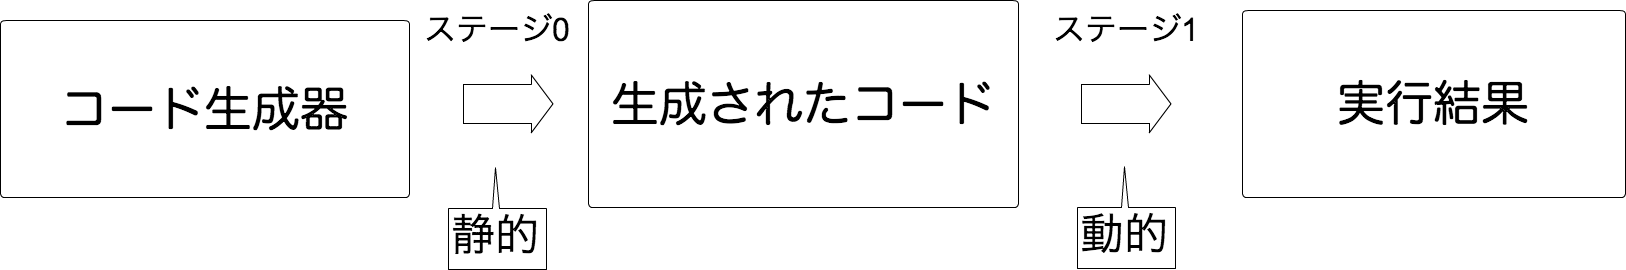
\includegraphics[clip,width=12cm]{./img/prggen.png}
  % この図を少し変更する
  \begin{itemize}
  \item コード生成段階とコード実行段階
    % \item 生成前の段階で,生成後のコードの安全性を保証する
  \item[⇒] 段階的計算をサポートするプログラム言語 ⇒ コード生成言語
    % \item 生成するプログラムだけでなく,生成されたプログラムも型の整合性が静的に (生成前に) 保証される.
  \end{itemize}
\end{frame}

\subsection{コード生成の例}
\begin{frame}
  \frametitle{コード生成言語による記述例}

  \pause
  \begin{align*}
    \visible<1->{\text{コード生成器}} \visible<2->{&\too \text{生成されるコード}} \\
    \visible<3->{(\cint~ 3)} \visible<4->{&\too \code{3}} \\
    \visible<5->{(\cint~ 3)~ \cPlus~ (\cint~ 5)} \visible<6->{&\too \code{3 + 5}} \\
    \visible<7->{\cfun{x}{~x~ \cPlus~ (\cint~ 3)}} \visible<8->{&\too \code{\fun{x'}{x' + 3}}} \\
    \visible<9->{\cfordo{x = \cdots}{\cdots}~ \cdots} 
\visible<10->{&\too \code{\fordo{x' = \cdots}{\cdots}~ \cdots}}
  \end{align*}

  \begin{visibleenv}<11>
    \begin{exampleblock}{コードコンビネータ}
      \begin{itemize}
      \item 下線つきの演算子
      \item コードを引数にとり、コードを返す
      \end{itemize}
    \end{exampleblock}
  \end{visibleenv}

  % \begin{align*}
      %       \fix f = f (\fix f) \\
      %       \cfordo{x = n}{m}~ e \to \code{\fordo{x = n}{m}~ e}
      %     \end{align*}
\end{frame}


\begin{frame}
  \frametitle{power関数のコード化}
  \begin{onlyenv}<1>
    普通のpower関数
    \begin{align*}
      \text{power} =~ &\lam x.~\fix~ \lam f. \lam n. \\
                      &~~\iif~ n=0~ \then~  1 \\
                      &~~\eelse~ x~ \times~ (f~ (n - 1))
    \end{align*}
  \end{onlyenv}

  \begin{onlyenv}<2->
    \texttt{gen\_power}: powerコード生成器
    \begin{align*}
      \text{gen\_power} =~ &\clam x. \fix~ \lam f. \lam n. \\
                           &\iif~ n=0~ \then~ (\cint~ 1) \\
                           &\eelse~ x~ \cTimes~ (f~ (n - 1))
    \end{align*}
  \end{onlyenv}

  \pause
  \pause
  $n = 5$に特化したコード生成:
  \pause
  \begin{align*}
    \cfun{x}{~\text{gen\_power}~ x~ 5} \too \code{\fun{x'}{~x' 
\times x' \times x' \times x' \times x' \times 1}}
  \end{align*}
  \pause
  gen\_power 関数によって生成されたコードは power 関数より高速
  \begin{itemize}
  \item 関数呼び出しがない
  \item 条件式がない
  \end{itemize}
\end{frame}

% \begin{frame}
%   \frametitle{従来研究}
%   \begin{itemize}
%   \item コード生成プログラムが,安全なコードのみを生成する事を静的に保証
%     %   \item<2-> let挿入等を実現する\alert{計算エフェクトを含む場合の安全性保証の研究は未整備}
%   \item 安全なコード: 構文,型,変数束縛が正しいプログラム
%   \end{itemize}

%   \pause

%   しかし\alert{多段階let挿入}等を実現する\alert{計算エフェクト}を含む場合のコード生成の安全性保証は研究途上
% \end{frame}

% 多段階let挿入というのはあるlet式をn個以上の束縛を抜けて任意の場所へ挿入するということ.
%
% 実際にはtの値によって挿入したい箇所が変わってくる.
% tの値によっては安全じゃない場合があるので,それは型が付かないようにしたい.
% そのような型による項の安全性を考えたい

\begin{frame}
  \frametitle{多段階let挿入}
                             %                              入れ子になったforループなどを飛び越えたコード移動を許す仕組みであり、ループ不変式の移動によって,効率的なコード生成に必要なプログラム技法

  \begin{itemize}
  \item 入れ子になったforループなどを飛び越えた\alert{コード移動}を許す仕組み
  \item ループ不変式の移動によって,\alert{効率的なコード生成}に必要なプログラミング技法
  \end{itemize}
\end{frame}

\begin{frame}[fragile]
  \frametitle{二重forループのコード生成例}
  コード生成器
  \begin{align*}
    & \cfordo{x = (\cint~0)}{(\cint~n)} \\
    & ~~\cfordo{y = (\cint~0)}{(\cint~m)} \\
    & ~~~~~~\caryset{a}{(x,y)}{(x ~\cPlus~ \text{complex calculation})} 
  \end{align*}

  \begin{visibleenv}<2>
    \begin{center}
      \LARGE \downtoo
    \end{center}
    生成されるコード
    \begin{align*}
      &\cbra~ \fordo{x' = 0}{n} \\
      & ~~~~\fordo{y' = 0}{m} \\
      & ~~~~~~\aryset{a}{x',y'}{(x' + \text{complex calculation})}~ \cket
    \end{align*}
  \end{visibleenv}
\end{frame}

\begin{frame}
  \frametitle{多段階let挿入}
  生成されるコード
  \begin{align*}
    \visible<4-5>{&\cbra~ \Let ~u = \red{\text{complex calculation}}~ \In \visible<5>{\footnotesize\blue{\text{  --- u が x' にも y' にも依存しない式 }}} \\}
                  &\visible<1-3>{\cbra~} \fordo{x' = 0}{n} \\
    \visible<2-3>{& ~~~~\Let ~u = \red{\text{complex calculation}}~ \In \visible<3>{\footnotesize\blue{\text{  --- u が x' にのみ依存し y' には依存しない式 }}} \\}
                  & ~~~~\fordo{y' = 0}{m} \\
    \\
                  & ~~~~~~\aryset{a}{x',y'}{x' + \visible<2->{u}~ \visible<1>{\red{\text{complex calculation}}}} \cket
  \end{align*}
\end{frame}

\begin{frame}
  \center
  \huge{そのような多段階のlet挿入をどうやって行うか}
\end{frame}

\begin{frame}
  \frametitle{多段階let挿入}
  コード生成器
  \begin{align*}
    & \visible<2->{\red{...}~} \cfordo{x = 0}{n} \\
    & \visible<2->{~~\red{...}~} \cfordo{y = 0}{m} \\
    & \visible<2->{~~~~\red{...}~} \cLet~u= \text{complex calculation}~\cIn \\
    & \visible<2->{~~~~~~\red{...}~} (\caryset{\code{a}}{(x,y)}{(i + u)})
  \end{align*}

  \begin{onlyenv}<3>
    \begin{exampleblock}{コントロールオペレータshift0/reset0の導入}
      $\red{...}$ のところに後に説明する shift0/reset0 というコントロールオペレータを用いることで,多段階let挿入を行う
    \end{exampleblock}
  \end{onlyenv}
\end{frame}

% やりたいことは,このような多段階let挿入をコード生成の前の段階で静的に安全性の保証を行うということ.

\begin{frame}
  \center
  \huge{危険な例}
\end{frame}


\begin{frame}[fragile]
  \frametitle{危険なコード生成の例}
  コード生成器
  \begin{align*}
    & \red{...}~ \cfordo{x = 0}{n} \\
    & ~~\red{...}~ \cfordo{y = 0}{m} \\
    & ~~~~\red{...}~ \magenta {\cLet~u= \text{complex calculation}~\cIn} \\
    & ~~~~~~\red{...}~ (\caryset{\code{a}}{(x,y)}{(i + u)})
  \end{align*}

  \begin{onlyenv}<2>
    \begin{center}
      \downtoo
    \end{center}
    生成されるコード
    \begin{align*}
      &\cbra~ \magenta{\Let ~u = \text{complex calculation}~ \In} \footnotesize\blue{\text{  --- u が x にも y にも依存する式 }} \\
      & ~~\fordo{x = 0}{n} \\
      & ~~~~\fordo{y = 0}{m} \\
      & ~~~~~~\aryset{a}{x,y}{(x + u)}~ \cket
    \end{align*}
  \end{onlyenv}

  \begin{onlyenv}<3>
    \begin{exampleblock}{complex calculation によって挿入できる場所が異なる}
      \begin{itemize}
      \item 多段階let挿入が可能となっても,安全に挿入できる場所とそうでない場所がある
      \item 安全にlet挿入を行うためにどうすればよいかを考える必要がある
      \end{itemize}
    \end{exampleblock}
  \end{onlyenv}
\end{frame}


% \begin{frame}
%   \frametitle{危険な例}
%   \begin{align*}
%     & \fordo{i = 0}{n} \\
%     & ~~\fordo{j = 0}{m} \\
%     & ~~~~\magenta{\Let ~y ~= ~a[i] + b[j] ~\In} ~~\tiny{\text{--- t がi,j に依存した式 }} \\
%     & ~~~~~~\aryset{a}{i,j}{b[i] + y} \\
%   \end{align*}

%   \begin{invisibleenv}<1>
%     \begin{center}
%       多段階let挿入\\
%       $\Downarrow$
%     \end{center}
%     \begin{align*}
%       & \magenta{\Let ~y ~= ~a[i] + b[j] ~\In} ~~\tiny{\text{--- t がi,j に依存した式 }} \\
%       & ~~\fordo{i = 0}{n} \\
%       & ~~~~\fordo{j = 0}{m} \\
%       & ~~~~~~\aryset{a}{i,j}{b[i] + y} \\
%     \end{align*}
%   \end{invisibleenv}

%   \begin{onlyenv}<2>
%     \begin{center}
%       多段階let挿入\\
%       $\Downarrow$
%     \end{center}
%     \begin{align*}
%       & \magenta{\Let ~y ~= ~a[i] + b[j] ~\In} \\
%       & ~~\fordo{i = 0}{n} \\
%       & ~~~~\fordo{j = 0}{m} \\
%       & ~~~~~~\aryset{a}{i,j}{b[i] + y} \\
%     \end{align*}
%   \end{onlyenv}
% \end{frame}

\subsection{段階的計算の課題}

\begin{frame}
  \frametitle{コード生成の利点と課題}
  利点
  \begin{itemize}
  \item \alert{「保守性・再利用性の高さ」}と\alert{「実行性能の高さ」}の両立
  \end{itemize}

  \pause

  課題
  \begin{itemize}
  \item パラメータに応じて,非常に多数のコードが生成される
    % \item 構文的,意味的に正しくないプログラムを生成しやすい
  \item 生成したコードのデバッグが容易ではない
  \item [⇒] \alert{コード生成の前に安全性を保証}したい
  \end{itemize}
\end{frame}

      %       \subsection{限定継続}

      %       \begin{frame}
      %       \frametitle{コントロールオペレータ}
      %       \begin{block}{プログラミング言語におけるプログラムを制御するプリミティブ}
      %       \begin{itemize}
      %       \item exception (例外): C++, Java, ML
      %       \item call/cc (第一級継続): Scheme, SML/NJ
      %       \item shift/reset (限定継続): Racket, Scala, OCaml
      %       \begin{itemize}
      %       \item 1989年以降多数研究がある
      %       \item コード生成におけるlet挿入が実現可能
      %         %       \item shift/reset + コード生成の型システムが幾つか提案されている
      %       \end{itemize}
      %       \item \alert{shift0/reset0}
      %       \begin{itemize}
      %       \item 2011年以降研究が活発化.
      %       \item コード生成における\alert{多段階let挿入}が可能
      %       \end{itemize}
      %       \end{itemize}
      %       \end{block}
      %       \end{frame}

      %%%       Local Variables:
      %%%       mode: japanese-latex
      %%%       TeX-master: "slide"
      %%%       End:
